\documentclass[conference]{IEEEtran}
\IEEEoverridecommandlockouts

\usepackage{cite}
\usepackage{amsmath,amssymb,amsfonts}
\usepackage{algorithmic}
\usepackage{graphicx}
\usepackage{textcomp}
\usepackage{xcolor}
\def\BibTeX{{\rm B\kern-.05em{\sc i\kern-.025em b}\kern-.08em
    T\kern-.1667em\lower.7ex\hbox{E}\kern-.125emX}}
\begin{document}

\title{Hybrid Model Predictive and Nonlinear Feedback Control for Chaos Suppression and MPPT Enhancement in DFIG-Based Wind Energy Systems}

\author{\IEEEauthorblockN{Said Regani}
\IEEEauthorblockA{\textit{L2EI Laboratory} \\
\textit{Jijel University}\\
BP 98 Ouled Aissa, Jijel 18000, Algeria}
\and
\IEEEauthorblockN{Manal Messadi}
\IEEEauthorblockA{\textit{L2EI Laboratory} \\
\textit{Jijel University}\\
BP 98 Ouled Aissa, Jijel 18000, Algeria}
\and
\IEEEauthorblockN{Kemih Karim}
\IEEEauthorblockA{\textit{L2EI Laboratory} \\
\textit{Jijel University}\\
BP 98 Ouled Aissa, Jijel 18000, Algeria}
}

\maketitle

\begin{abstract}
Doubly fed induction generator (DFIG)-based wind turbines are strongly nonlinear electromechanical systems that can exhibit chaotic dynamics under perturbed parameters and adverse operating conditions, leading to degraded power quality and compromised stability. This paper analyses a third-order rotor-current/speed model of the DFIG with a physically consistent parameter set, characterizes its equilibria, dissipativity and Lyapunov exponents, and proposes a hybrid controller acting only on the two rotor voltages. An outer speed loop generates the torque-current reference, nonlinear feedback compensation cancels the coupled current dynamics, and a constrained receding-horizon Model Predictive Control (MPC) with integral action, whose terminal weight and gain are obtained from a linear matrix inequality, handles the converter voltage limits. Simulations show that the controller suppresses the chaotic oscillations within 0.13~s without steady-state error, and tracks Maximum Power Point Tracking (MPPT) references under turbulent wind with a speed RMS error of 0.008~rad/s and a stator-power RMS error below 1\,\% of the mean power.
\end{abstract}

\begin{IEEEkeywords}
Doubly-Fed Induction Generator (DFIG), Wind Energy Systems, Chaotic Dynamics, Nonlinear Dynamics, Maximum Power Point Tracking (MPPT), Hybrid Control, Model Predictive Control (MPC), Nonlinear Feedback Control.
\end{IEEEkeywords}

\section{Introduction}

The escalating global population coupled with increasing electricity demand has accelerated the depletion of non-renewable energy resources at unprecedented rates \cite{b1}. This critical challenge necessitates the exploration and deployment of alternative, sustainable, and environmentally-friendly energy sources, particularly wind energy, to mitigate environmental degradation and address energy security concerns \cite{b2}, \cite{b3}.

Wind energy has emerged as a pivotal renewable energy technology in recent decades, experiencing substantial growth in both global investments and installed capacity \cite{b4}. Recent statistics indicate that global wind power capacity expanded by a record 117 GW in 2024, elevating the cumulative worldwide installed capacity to approximately 1,136 GW \cite{b5}. This remarkable expansion has been driven by supportive policy frameworks, technological innovations, and declining levelized cost of energy, positioning wind power as one of the fastest-growing renewable energy sources worldwide \cite{b6}.

Among various wind turbine generator configurations, the doubly fed induction generator (DFIG) has become the dominant technology in large-scale onshore wind farms, primarily due to its partial-scale back-to-back power converter architecture that enables flexible control of active and reactive power with reduced converter ratings \cite{b7}, \cite{b8}. This configuration allows the rotor-side converter (RSC) and grid-side converter (GSC) to independently regulate rotor currents and grid-injected currents, respectively, thereby achieving decoupled control of electromagnetic torque, stator active power, and reactive power over a wide operational speed range \cite{b9}.

The economic advantage of requiring only 25--30\% rated power converters compared to full-scale converter systems, combined with superior power quality and grid-support capabilities, has made DFIG the preferred choice for variable-speed wind energy conversion systems (WECS) \cite{b10}.

Despite extensive research on DFIG-based WECS including dynamic modeling, vector control strategies, grid-fault ride-through capability, and ancillary services provision, recent studies have revealed that these systems can exhibit complex nonlinear dynamic behaviors under certain operating conditions \cite{b11}--\cite{b13}. The inherent nonlinearity of the induction machine, coupled with the interaction between mechanical and electrical subsystems and the coupling between stator and rotor flux linkages, can lead to oscillatory transients and, under severe conditions, bifurcations and quasi-chaotic responses \cite{b14}, \cite{b15}.

These phenomena become particularly pronounced under severe grid disturbances, highly turbulent wind speed profiles, parameter uncertainties (such as machine detuning), and converter saturation effects, all of which may degrade power quality, stress mechanical components, and compromise system stability \cite{b16}, \cite{b17}.

The emergence of chaotic behavior in DFIG systems manifests as irregular power oscillations, torque ripple, and complex trajectories in the state space, which are detrimental to both electrical and mechanical performance \cite{b18}. Such dynamics are especially critical in the context of stringent grid-code requirements for low-voltage ride-through (LVRT), frequency support, and reactive power support \cite{b19}, \cite{b20}.

Consequently, the analysis, mitigation, and control of nonlinear and potentially chaotic dynamics in DFIG-based wind turbines have become important research priorities for ensuring stable operation under wide-ranging operating scenarios and maximizing the contribution of wind energy to global electricity supply.

Motivated by these challenges, this paper investigates the control of a variable-speed wind turbine equipped with a DFIG that exhibits chaotic-like behavior induced by machine parameter deviations and adverse operating scenarios, which can severely affect system stability and grid-injected power quality. A comprehensive nonlinear mathematical model is first developed to capture the intricate coupling among rotor currents, electromagnetic torque, and mechanical speed, and to identify the conditions under which complex or chaotic regimes emerge when the system is subjected to significant disturbances, such as abrupt wind-speed variations or degraded parameter settings. Moreover, the system is subjected to a highly realistic wind-speed profile to evaluate its ability to maintain stability and drive its dynamics toward accurate wind-path tracking, as assessed through the tracking error. Building on this framework, an innovative hybrid control architecture is then proposed, combining Model Predictive Control (MPC) with nonlinear state-feedback compensation to suppress chaotic dynamics and achieve high-precision tracking of reference rotor current and speed trajectories derived from Maximum Power Point Tracking (MPPT) objectives.

\section{Wind Turbine Modeling}

The aerodynamic power captured by a horizontal-axis wind turbine can be written as \cite{b21,b22,b23}
\begin{equation}
P_{a} = \frac{1}{2}\pi\rho R^{2}C_{p}(\lambda)\, v^{3}
\label{eq1}
\end{equation}
where $\rho$ is the air density, $R$ is the rotor radius, $v$ is the wind speed, and $C_{p}(\lambda)$ is the power coefficient, which depends on the tip-speed ratio $\lambda$.

The tip-speed ratio is defined by
\begin{equation}
\lambda = \frac{R\omega_{r}}{v}
\label{eq2}
\end{equation}
with $\omega_{r}$ the rotor (mechanical) angular speed.

The corresponding aerodynamic torque applied to the shaft is obtained from
\begin{equation}
T_{a} = \frac{P_{a}}{\omega_{r}} = \frac{1}{2}\pi\rho R^{2}C_{p}(\lambda)\,\frac{v^{3}}{\omega_{r}}
\label{eq3}
\end{equation}

The rotational dynamics of the wind turbine--generator set are described by
\begin{equation}
J\frac{d\Omega_{m}}{dt} = T_{a} - T_{e} - D\Omega_{m}
\label{eq4}
\end{equation}
where $J$ is the total inertia, $\Omega_{m}$ is the mechanical rotor speed, $T_{e}$ is the electromagnetic torque produced by the generator, and $D$ denotes the viscous friction coefficient.

Relating mechanical and electrical rotor speeds by
\begin{equation}
\omega_{r} = n_{p}\Omega_{m}
\label{eq5}
\end{equation}
with $n_{p}$ the number of pole pairs, and using $\frac{d\Omega_{m}}{dt} = \frac{1}{n_{p}}\frac{d\omega_{r}}{dt}$, \eqref{eq4} can be rewritten in electrical speed form as
\begin{equation}
\frac{J}{n_{p}}\frac{d\omega_{r}}{dt} = T_{a} - T_{e} - \frac{D}{n_{p}}\omega_{r}
\label{eq6}
\end{equation}

For a DFIG expressed in the stator $dq$ reference frame, the electromagnetic torque is given by
\begin{equation}
T_{e} = \frac{3}{2}n_{p}\left( \psi_{ds}i_{qs} - \psi_{qs}i_{ds} \right)
\label{eq7}
\end{equation}
where $\psi_{ds},\psi_{qs}$ are the stator flux components and $i_{ds},i_{qs}$ are the corresponding stator current components.

Substituting \eqref{eq7} into \eqref{eq6} yields the final electromechanical dynamic equation of the rotor:
\begin{equation}
\frac{J}{n_{p}}\frac{d\omega_{r}}{dt} = T_{a} - \frac{3}{2}n_{p}\left( \psi_{ds}i_{qs} - \psi_{qs}i_{ds} \right) - \frac{D}{n_{p}}\omega_{r}
\label{eq8}
\end{equation}

\section{Chaotic Doubly-Fed Induction Generator}

According to \eqref{eq8} and the stator-flux/rotor-current coupling of the DFIG, a third-order state equation with $i_{dr}$, $i_{qr}$, and $\omega_{r}$ as state variables can be obtained \cite{b24}:
\begin{equation}
\begin{aligned}
\dot{i}_{dr} &= \left( - \frac{R_{s}L_{m}^{2}}{\sigma L_{s}^{2}L_{r}} - \frac{R_{r}}{\sigma L_{r}} \right)i_{dr} + \left( \omega_{s} - \omega_{r} \right)i_{qr} \\
&\quad- \frac{\omega_{r}L_{m}\psi_{s}}{\sigma L_{r}L_{s}} + \left( - \frac{L_{m}}{\sigma L_{s}L_{r}} \right)u_{ds} + \frac{1}{\sigma L_{r}}u_{dr} \\[4pt]
\dot{i}_{qr} &= - \left( \omega_{s} - \omega_{r} \right)i_{dr} + \left( - \frac{R_{s}L_{m}^{2}}{\sigma L_{s}^{2}L_{r}} - \frac{R_{r}}{\sigma L_{r}} \right)i_{qr} \\
&\quad+ \frac{R_{s}L_{m}\psi_{s}}{\sigma L_{s}^{2}L_{r}} + \left( - \frac{L_{m}}{\sigma L_{s}L_{r}} \right)u_{qs} + \frac{1}{\sigma L_{r}}u_{qr} \\[4pt]
\dot{\omega}_{r} &= \left( \frac{n_{p}}{J} \right)\left( \frac{3n_{p}L_{m}\psi_{s}}{2L_{s}}\, i_{dr} - \frac{D}{n_{p}}\omega_{r} - T_{L} \right)
\end{aligned}
\label{eq9}
\end{equation}

We now rewrite \eqref{eq9} by introducing the following state variables:
\begin{equation*}
x_{1} = i_{dr},\quad x_{2} = i_{qr},\quad x_{3} = \omega_{r}.
\end{equation*}

Let the parameters $a_{1},a_{2},\ldots,a_{8}$ be defined accordingly. The resulting nonlinear system can then be expressed in the compact state-space form
\begin{equation}
\left\{ \begin{aligned}
\dot{x}_{1} &= a_{1}x_{1} + \left( \omega_{s} - x_{3} \right)x_{2} + a_{2}x_{3} + \left( a_{3}u_{ds} + a_{4}u_{dr} \right), \\
\dot{x}_{2} &= - \left( \omega_{s} - x_{3} \right)x_{1} + a_{1}x_{2} + a_{5} + \left( a_{3}u_{qs} + a_{4}u_{qr} \right), \\
\dot{x}_{3} &= a_{6}x_{1} - a_{7}x_{3} - a_{8}.
\end{aligned} \right.
\label{eq10}
\end{equation}

The coefficients appearing in \eqref{eq10} are given by
\begin{equation*}
\begin{gathered}
a_{1} = - \frac{R_{s}L_{m}^{2}}{\sigma L_{s}^{2}L_{r}} - \frac{R_{r}}{\sigma L_{r}},\quad a_{2} = - \frac{L_{m}\psi_{s}}{\sigma L_{r}L_{s}},\quad a_{3} = - \frac{L_{m}}{\sigma L_{s}L_{r}},\\
a_{4} = \frac{1}{\sigma L_{r}},\quad a_{5} = \frac{R_{s}L_{m}\psi_{s}}{\sigma L_{s}^{2}L_{r}},\quad
a_{6} = \frac{3n_{p}^{2}L_{m}\psi_{s}}{2JL_{s}},\\ a_{7} = \frac{D}{J},\quad a_{8} = \frac{n_{p}}{J}T_{L},
\end{gathered}
\end{equation*}
with $\sigma = 1 - L_{m}^{2}/(L_{s}L_{r})$. The stator flux is aligned with the $q$ axis, so that $u_{ds} = -\omega_{s}\psi_{s}$ and $u_{qs} = 0$.

\begin{table}[htbp]
\caption{Main Parameters of the Chaotic DFIG System}
\begin{center}
\begin{tabular}{|c|c||c|c|}
\hline
\textbf{Parameter} & \textbf{Value} & \textbf{Parameter} & \textbf{Value} \\
\hline
$R_{s}$ & $5.0536 \times 10^{-5}\,\Omega$ & $n_{p}$ & $2$ \\
\hline
$R_{r}$ & $1.8781 \times 10^{-4}\,\Omega$ & $J$ & $31.18\,\text{kg}\cdot\text{m}^2$ \\
\hline
$L_{s}$ & $0.0833\,\text{H}$ & $D$ & $71.85\,\text{N}\cdot\text{m}\cdot\text{s/rad}$ \\
\hline
$L_{r}$ & $0.0844\,\text{H}$ & $T_{L}$ & $-11337\,\text{N}\cdot\text{m}$ \\
\hline
$L_{m}$ & $0.0811\,\text{H}$ & $u_{dr}$ & $2.539\,\text{V}$ \\
\hline
$\sigma$ & $0.0645$ & $u_{qr}$ & $-2.936\,\text{V}$ \\
\hline
$\omega_{s}$ & $100\pi\,\text{rad/s}$ & $u_{ds}$ & $-563.4\,\text{V}$ \\
\hline
$\psi_{s}$ & $1.7933\,\text{Wb}$ & $u_{qs}$ & $0\,\text{V}$ \\
\hline
\end{tabular}
\label{tab1}
\end{center}
\end{table}

The parameters listed in Table~\ref{tab1} are physically consistent: $L_{s},L_{r}>L_{m}$ and $\sigma = 0.0645 \in (0,1)$. They give $a_{1} = -0.0433$, $a_{2} = -320.83$, $a_{3} = -178.91$, $a_{4} = 183.76$, $a_{5} = 0.1946$, $a_{6} = 0.3360$, $a_{7} = 2.3044$, $a_{8} = -727.20$. The constant terms of \eqref{eq10} are therefore $a_{3}u_{ds}+a_{4}u_{dr} = 1.0126\times10^{5}$ and $a_{5}+a_{3}u_{qs}+a_{4}u_{qr} = -539.32$.

System \eqref{eq10} has three equilibrium points, all unstable:
\begin{itemize}
\item $E_{1} = (-64.94,\,-379.12,\,306.11)$, a saddle-focus with eigenvalues $1.462 \pm 7.673j$ and $-5.315$;
\item $E_{2} = (-9.97,\,-12442.5,\,314.12)$, a saddle with eigenvalues $-65.00$, $62.65$ and $-0.043$;
\item $E_{3} = (55.50,\,-272.00,\,323.67)$, a saddle-focus with eigenvalues $0.547 \pm 10.511j$ and $-3.486$.
\end{itemize}
The divergence of the vector field is constant and negative, $\nabla\cdot f = 2a_{1} - a_{7} = -2.391$, so the system is dissipative.

With these parameters, the dynamical system exhibits complex nonlinear behavior. The corresponding chaotic attractors generated from the initial condition $x(0) = (0.3,\, 0.6,\, 3.6)^{T}$ are illustrated in Fig.~\ref{fig1}.

\begin{figure}[htbp]
\centerline{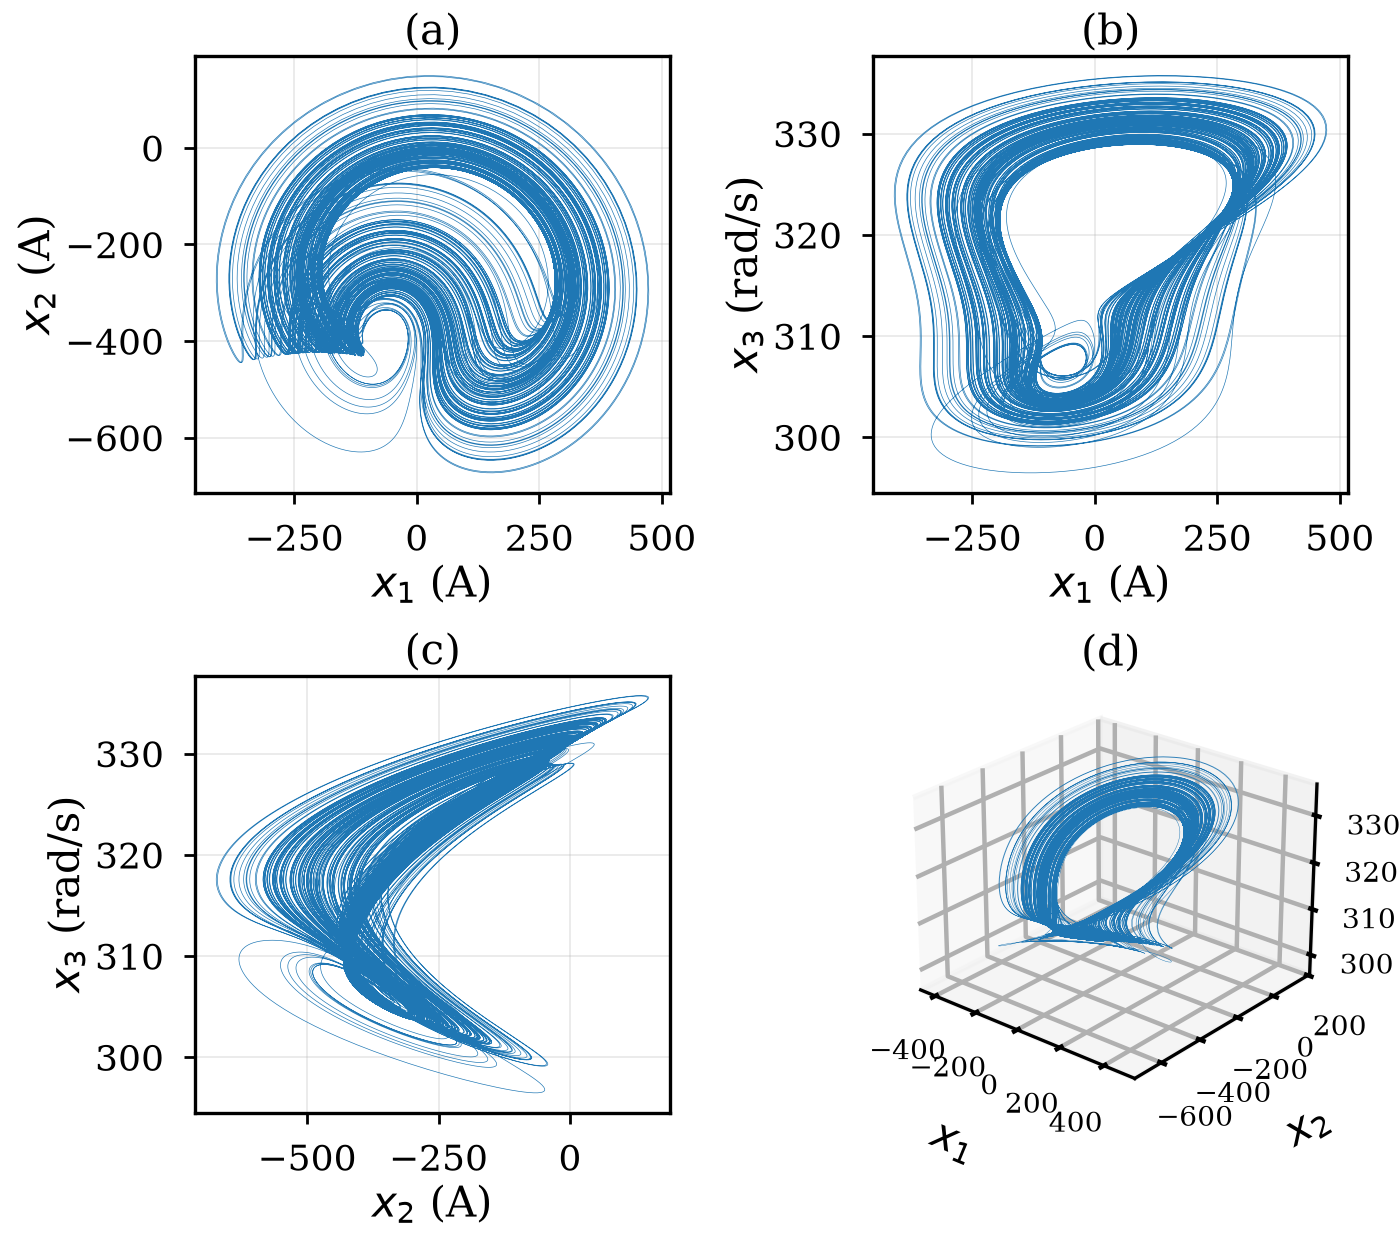
\includegraphics[width=0.48\textwidth]{fig1.png}}
\caption{The chaotic attractors: a) The projection of the chaotic attractor in plan $x_{1}-x_{2}$; b) the projection of the chaotic attractor in plan $x_{1}-x_{3}$; c) the projection of the chaotic attractor in plan $x_{2}-x_{3}$; d) 3D trajectory of the system.}
\label{fig1}
\end{figure}

The phase portraits presented in Fig.~\ref{fig1} illustrate the complex nonlinear behavior of the DFIG system. The trajectory winds around the two saddle-foci $E_{1}$ and $E_{3}$. The rotor speed remains positive and close to synchronism ($296 \le \omega_{r} \le 336$~rad/s), while the rotor currents oscillate irregularly between about $-670$ and $+470$~A. The Lyapunov exponents, computed with the QR-based variational method, are $(0.202,\,-0.010,\,-2.582)$. Their sum equals the divergence $-2.391$, and the Kaplan--Yorke dimension is $2.08$. The positive largest Lyapunov exponent confirms the presence of chaotic dynamics. The three-dimensional attractor further highlights the bounded yet aperiodic evolution of the system states, which is a typical signature of chaos.

\section{Reference Trajectory Generation and Tracking Error Formulation}

A realistic wind excitation is essential for evaluating the dynamic performance of a DFIG-based wind energy conversion system. In this work, the wind speed is modeled as the combination of a mean component, several low-frequency harmonic components, and a stochastic turbulence term, yielding a physically representative turbulent wind signal. The wind-speed model is expressed as
\begin{equation}
v(t) = V_{mean} + \sum_{k = 1}^{3}A_{k}\sin\left( 2\pi f_{k}t \right) + v_{turb}(t)
\label{eq11}
\end{equation}
here $V_{mean}$ denotes the average wind speed, $A_{k}$ and $f_{k}$ are the amplitudes and frequencies of the harmonic components, and $v_{turb}(t)$ is a smoothed Gaussian noise process representing atmospheric turbulence.

\begin{figure}[htbp]
\centerline{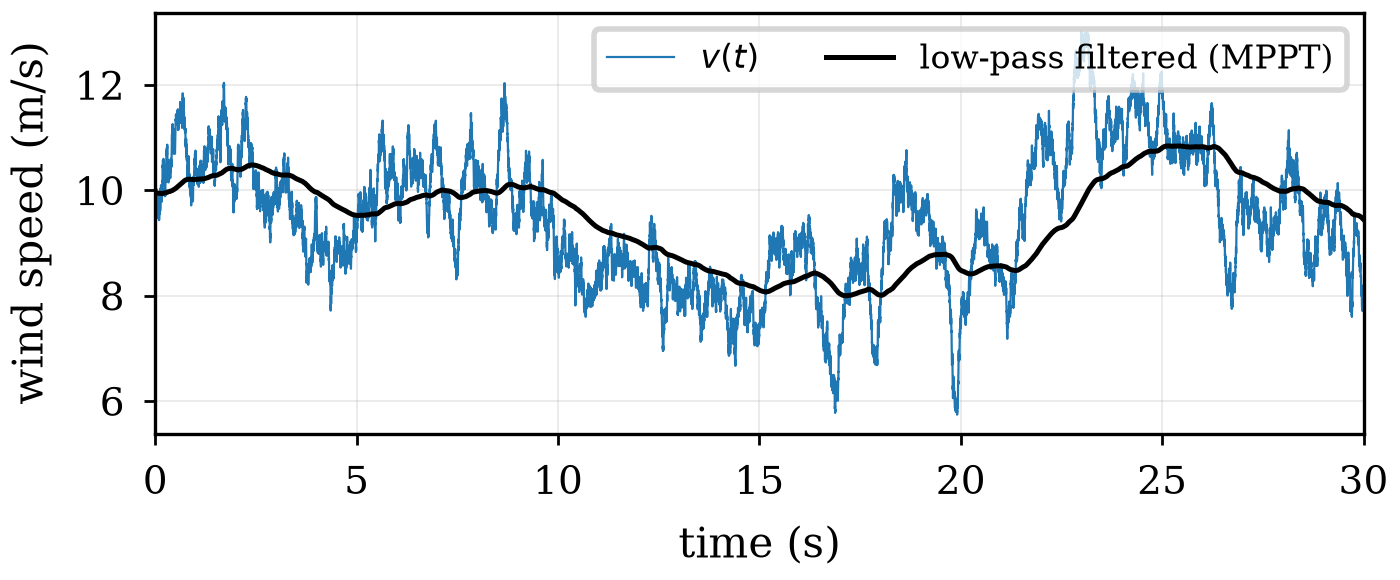
\includegraphics[width=0.48\textwidth]{fig2.png}}
\caption{Wind-speed trajectory.}
\label{fig2}
\end{figure}

Fig.~\ref{fig2} shows the generated wind-speed profile used to excite the DFIG system. The signal combines deterministic low-frequency variations with stochastic turbulence, providing a realistic representation of wind conditions. This complex excitation plays a key role in revealing the nonlinear and potentially chaotic behavior of the system.

Based on this profile, the aerodynamic power reference is computed from the standard wind-power expression
\begin{equation}
P_{ref}(t) = \frac{1}{2}\rho\pi R^{2}C_{p}v^{3}(t)
\label{eq12}
\end{equation}
where $\rho$ is the air density, $R$ the turbine radius, and $C_{p}$ the optimal power coefficient. With the stator flux aligned with the $q$ axis (Section~III), the electromagnetic torque and the stator active power are governed by the $d$-axis rotor current, leading to the reference
\begin{equation}
i_{dr,ref}(t) = -\frac{2}{3}\,\frac{P_{ref}(t)}{V_{s}}\,\frac{L_{s}}{L_{m}}
\label{eq13}
\end{equation}

The corresponding measured active power is
\begin{equation}
P_{m}(t) = -\frac{3}{2}\,\frac{L_{m}}{L_{s}}V_{s}i_{dr}(t)
\label{eq14}
\end{equation}

The reference for the $q$-axis rotor current is derived from the stator reactive-power expression under stator-flux orientation,
\begin{equation}
i_{qr,ref}(t) = - \,\frac{2L_{s}}{3L_{m}V_{s}}\left( Q_{s}(t) - \frac{3V_{s}^{2}}{2\omega_{s}L_{s}} \right)
\label{eq15}
\end{equation}
and, by imposing $Q_{s}(t) = 0$, simplifies to the constant operating point
\begin{equation}
i_{qr,ref} = \frac{V_{s}}{\omega_{s}L_{m}} = \frac{\psi_{s}}{L_{m}}
\label{eq16}
\end{equation}
which ensures unity power-factor operation.

The reference rotor speed is obtained from the optimal tip-speed ratio, giving
\begin{equation}
\omega_{r,ref}(t) = \frac{G\,\lambda_{opt}}{R}\, v(t)
\label{eq17}
\end{equation}

The complete reference trajectory is therefore
\begin{equation*}
x_{r}(t) = \begin{bmatrix}
i_{dr,ref}(t) \\
i_{qr,ref}(t) \\
\omega_{r,ref}(t)
\end{bmatrix},
\end{equation*}
and the corresponding tracking errors are defined as
\begin{equation*}
e(t) = x(t) - x_{r}(t),\quad e_{i}(t) = x_{i}(t) - x_{r,i}(t),\quad i = 1,2,3.
\end{equation*}

A common practice in addressing the control problem of wind turbines is to use a linearization approach. However, due to the stochastic operating conditions and the inevitable uncertainties inherent in the system, such control methods come at the price of poor system performance and low reliability. Hence the need for nonlinear control to take into account these control problems.

\section{Hybrid Control of a Novel Chaotic DFIG-Based System}

The controlled system takes the form
\begin{equation}
\begin{aligned}
\dot{x}_{1} &= a_{1}x_{1} + \left( \omega_{s} - x_{3} \right)x_{2} + a_{2}x_{3} + a_{3}u_{ds} + a_{4}u_{1}, \\
\dot{x}_{2} &= - \left( \omega_{s} - x_{3} \right)x_{1} + a_{1}x_{2} + a_{5} + a_{3}u_{qs} + a_{4}u_{2}, \\
\dot{x}_{3} &= a_{6}x_{1} - a_{7}x_{3} - a_{8},
\end{aligned}
\label{eq18}
\end{equation}
where $x = \left\lbrack x_{1},x_{2},x_{3} \right\rbrack^{T} = \left\lbrack i_{dr},i_{qr},\omega_{r} \right\rbrack^{T}$ and the two control inputs $u_{1} = u_{dr}$ and $u_{2} = u_{qr}$ are the rotor voltages imposed by the rotor-side converter. The speed equation has no direct input: $\omega_{r}$ is controlled through the electromagnetic torque, i.e., through $i_{dr}$. With the parameters of Table~\ref{tab1}, \eqref{eq18} reads
\begin{equation*}
\begin{aligned}
\dot{x}_{1} &= -0.0433\,x_{1} + \left( \omega_{s} - x_{3} \right)x_{2} - 320.83\,x_{3} \\
&\quad + 1.0079\times10^{5} + 183.76\,u_{1}, \\
\dot{x}_{2} &= - \left( \omega_{s} - x_{3} \right)x_{1} - 0.0433\,x_{2} + 0.1946 + 183.76\,u_{2}, \\
\dot{x}_{3} &= 0.3360\,x_{1} - 2.3044\,x_{3} + 727.20 .
\end{aligned}
\end{equation*}
In open loop ($u_{1} = 2.539$~V, $u_{2} = -2.936$~V), \eqref{eq18} reduces to the chaotic system \eqref{eq10}. The objective is to force the nonlinear chaotic dynamics to follow a desired trajectory $x_{d}(t)$, constructed from wind-profile-based references for $i_{dr}$, $i_{qr}$, and $\omega_{r}$. The tracking error is defined as $e(t) = x(t) - x_{d}(t)$, and its stabilization ensures both chaos suppression and accurate MPPT behavior under turbulent wind fluctuations.

The overall control structure implementing this hybrid strategy combining Model Predictive Control with nonlinear feedback compensation is illustrated in Fig.~\ref{fig3}, where the proposed controller interacts with the turbine dynamics and the MPPT block to achieve accurate trajectory tracking under variable wind conditions.

This hybrid framework harnesses the strengths of both techniques to overcome their individual limitations and improve overall system performance. Predictive control \cite{b25,b26,b27,b28,b29} is particularly valued for its ease of configuration and implementation, which makes it a widely adopted technique for controlling chaotic systems. Its efficiency and straightforward design process enable effective management of complex dynamics with relatively low computational effort. Feedback control excels in stabilizing inherently unstable and unpredictable chaotic dynamics by continuously adjusting the control input in real time based on the system's current state. Additionally, feedback control \cite{b30,b31,b32,b33} offers significant adaptability, allowing synchronization or steering of chaotic trajectories toward desired states, which is crucial for practical applications such as cryptography, robotics, and biological systems. By integrating these two approaches, the proposed hybrid control strategy capitalizes on the simplicity of predictive control alongside the real-time adaptability and energy efficiency of feedback control, thereby providing a more comprehensive solution for managing chaotic systems.

\begin{figure}[htbp]
\centerline{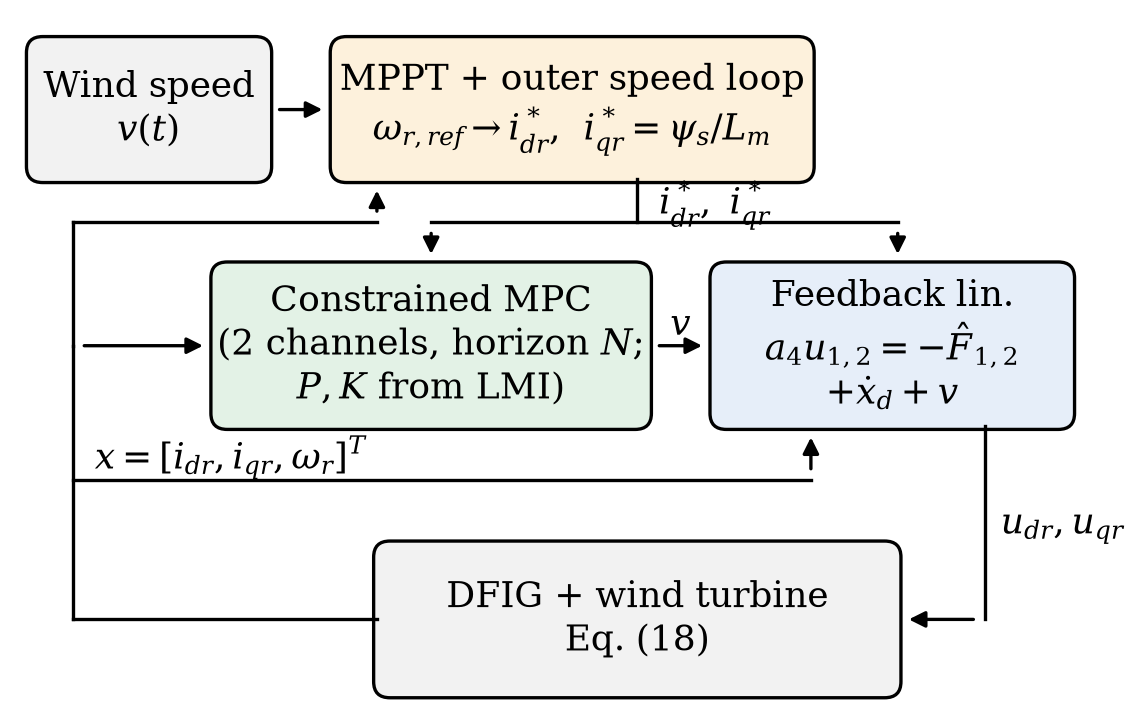
\includegraphics[width=0.46\textwidth]{fig3.png}}
\caption{Proposed hybrid MPC--nonlinear feedback control architecture: outer speed loop and inner current loops acting on the rotor voltages $u_{1}=u_{dr}$, $u_{2}=u_{qr}$.}
\label{fig3}
\end{figure}

\subsection{Outer Speed Loop}
Since $T_{e}\propto i_{dr}$, the speed is controlled through the reference of $i_{dr}$. With $e_{\omega}=\omega_{r}-\omega_{r,ref}$ and the nominal model,
\begin{equation}
i^{\ast}_{dr}=\frac{\dot\omega_{r,ref}+a_{7}\,\omega_{r,ref}+a_{8}-\lambda e_{\omega}-\lambda_{I}\!\int\! e_{\omega}\,dt}{a_{6}},
\label{eq19}
\end{equation}
where $a_{8}=n_{p}T_{L}/J$ uses the load (or aerodynamic) torque. Substituting \eqref{eq19} into the third line of \eqref{eq18} gives
\[
\dot e_{\omega}=-(\lambda+a_{7})\,e_{\omega}-\lambda_{I}\!\int\! e_{\omega}\,dt+a_{6}\,(i_{dr}-i^{\ast}_{dr}),
\]
an exponentially stable linear system driven by the inner tracking error; hence $e_{\omega}\to0$ once $i_{dr}\to i^{\ast}_{dr}$ (cascade argument). The inner reference is $x_{d}=[i^{\ast}_{dr},\,i_{qr,ref}]^{T}$ with $i_{qr,ref}=\psi_{s}/L_{m}$ from \eqref{eq16}.

\subsection{Inner Loop: Nonlinear Feedback Compensation}
Write the first two lines of \eqref{eq18} as $\dot x_{1,2}=F_{1,2}(x)+a_{4}u_{1,2}$ and let $\hat F_{1,2}$ be the nominal model. The control law
\begin{equation}
u_{1,2}=\frac{1}{a_{4}}\Big(-\hat F_{1,2}(x)+\dot x_{d}+v\Big)
\label{eq20}
\end{equation}
gives $\dot e=v+\Delta$, with $e=x_{1,2}-x_{d}$ and $\Delta=F_{1,2}-\hat F_{1,2}$ ($\Delta=0$ nominally). The bilinear couplings $(\omega_{s}-x_{3})x_{1,2}$ responsible for chaos are cancelled, leaving two decoupled integrators driven by $v$. Combining such a compensation with MPC has been shown effective for MPPT of wind turbines \cite{b34}.

\subsection{Model Predictive Control}
For each channel $i\in\{1,2\}$, the error is augmented with its integral, $\xi_{i}=[e_{i},\int e_{i}dt]^{T}$, and sampled with period $T_{s}$:
\begin{equation}
\xi_{i}(k+1)=A\xi_{i}(k)+Bv_{i}(k),\quad A=\begin{bmatrix}1&0\\T_{s}&1\end{bmatrix}\!,\ B=\begin{bmatrix}T_{s}\\T_{s}^{2}/2\end{bmatrix}\!.
\label{eq21}
\end{equation}
At each instant $k$, the MPC solves the quadratic program
\begin{equation}
\begin{aligned}
\min_{v_{i}(\cdot|k)}\ & \sum_{j=1}^{N}\|\xi_{i}(k+j|k)\|_{Q}^{2}+\|\xi_{i}(k+N|k)\|_{P}^{2}\\
& +r\sum_{j=0}^{N-1}v_{i}(k+j|k)^{2}\\
\text{s.t. }\ & \eqref{eq21},\qquad |u_{i}(k+j|k)|\le\bar u ,
\end{aligned}
\label{eq22}
\end{equation}
with prediction horizon $N$, weights $Q=Q^{T}>0$, $r>0$, and the converter voltage limit $\bar u$ (via \eqref{eq20}, a bound on $v_{i}$). Only the first optimal move is applied and the problem is solved again at $k+1$ (receding horizon) \cite{b35}; the integral is frozen when the limit is reached.

\textit{Theorem 1:} Let $X=X^{T}>0$ and $Y$ satisfy the LMI
\begin{equation}
\begin{bmatrix}
X & (AX+BY)^{T} & XQ^{1/2} & \sqrt{r}\,Y^{T}\\
AX+BY & X & 0 & 0\\
Q^{1/2}X & 0 & I & 0\\
\sqrt{r}\,Y & 0 & 0 & 1
\end{bmatrix}\succeq0,
\label{eq23}
\end{equation}
and set $P=X^{-1}$, $K=YX^{-1}$. Then $(A+BK)^{T}P(A+BK)-P+Q+rK^{T}K\preceq0$, and if \eqref{eq22}, augmented with the terminal constraint $\xi_{i}(k+N|k)\in\Omega=\{\xi^{T}P\xi\le\alpha\}$ ($\alpha$ such that $K\xi$ respects the limits in $\Omega$), is feasible at $k=0$ with $\Delta=0$, it remains feasible and $\xi_{i}=0$ is asymptotically stable.

\textit{Proof:} The Schur complement of \eqref{eq23} gives $X-(AX+BY)^{T}X^{-1}(AX+BY)-XQX-rY^{T}Y\succeq0$; pre- and post-multiplying by $P$ with $Y=KX$ yields the stated inequality. Thus $\xi^{T}P\xi$ is a Lyapunov function for $v=K\xi$ and $\Omega$ is invariant. By the standard terminal-cost argument \cite{b35}, the optimal cost decreases by at least $\|\xi_{i}(k)\|_{Q}^{2}+rv_{i}(k)^{2}$ at each step, which proves recursive feasibility and asymptotic stability. \hfill$\blacksquare$

\textit{Remark:} The LMI formulation of the terminal ingredients follows \cite{b36}. The maximal-volume solution of \eqref{eq23} is the Riccati solution, so without active constraints the MPC returns exactly $v_{i}=K\xi_{i}$: a single gain $K=[k_{e},k_{I}]$ from the LMI replaces the previous matrices $K_{1}$, $K_{2}$ and the diagonal $K$.

\section{Numerical Simulations}

All simulations integrate \eqref{eq18} with a fourth-order Runge--Kutta scheme (step $T_{s}/4$). The controller uses $T_{s}=1$~ms, $N=10$, $Q=\mathrm{diag}(1,3)$, $r=10^{-6}$ (currents scaled by 100~A), which gives $K=[-619.2,\,-1069.5]$ and an LMI residual below $10^{-15}$; the outer loop uses $\lambda=10$~s$^{-1}$, $\lambda_{I}=25$~s$^{-2}$, and the rotor voltages are limited to $|u_{dr}|,|u_{qr}|\le200$~V.

\subsection{Chaos Suppression}
The system starts from $x(0)=(0.3,0.6,3.6)^{T}$ with the open-loop voltages of Table~\ref{tab1} and evolves on the chaotic attractor. At $t=10$~s the controller is activated with the target $\omega_{r}^{\ast}=1.05\,\omega_{s}=329.9$~rad/s and $i_{qr}^{\ast}=\psi_{s}/L_{m}=22.1$~A ($Q_{s}=0$); the corresponding equilibrium $i_{dr}^{\ast}=98.0$~A is held with $u_{dr}=29.3$~V and $u_{qr}=-8.4$~V.

\begin{figure}[htbp]
\centerline{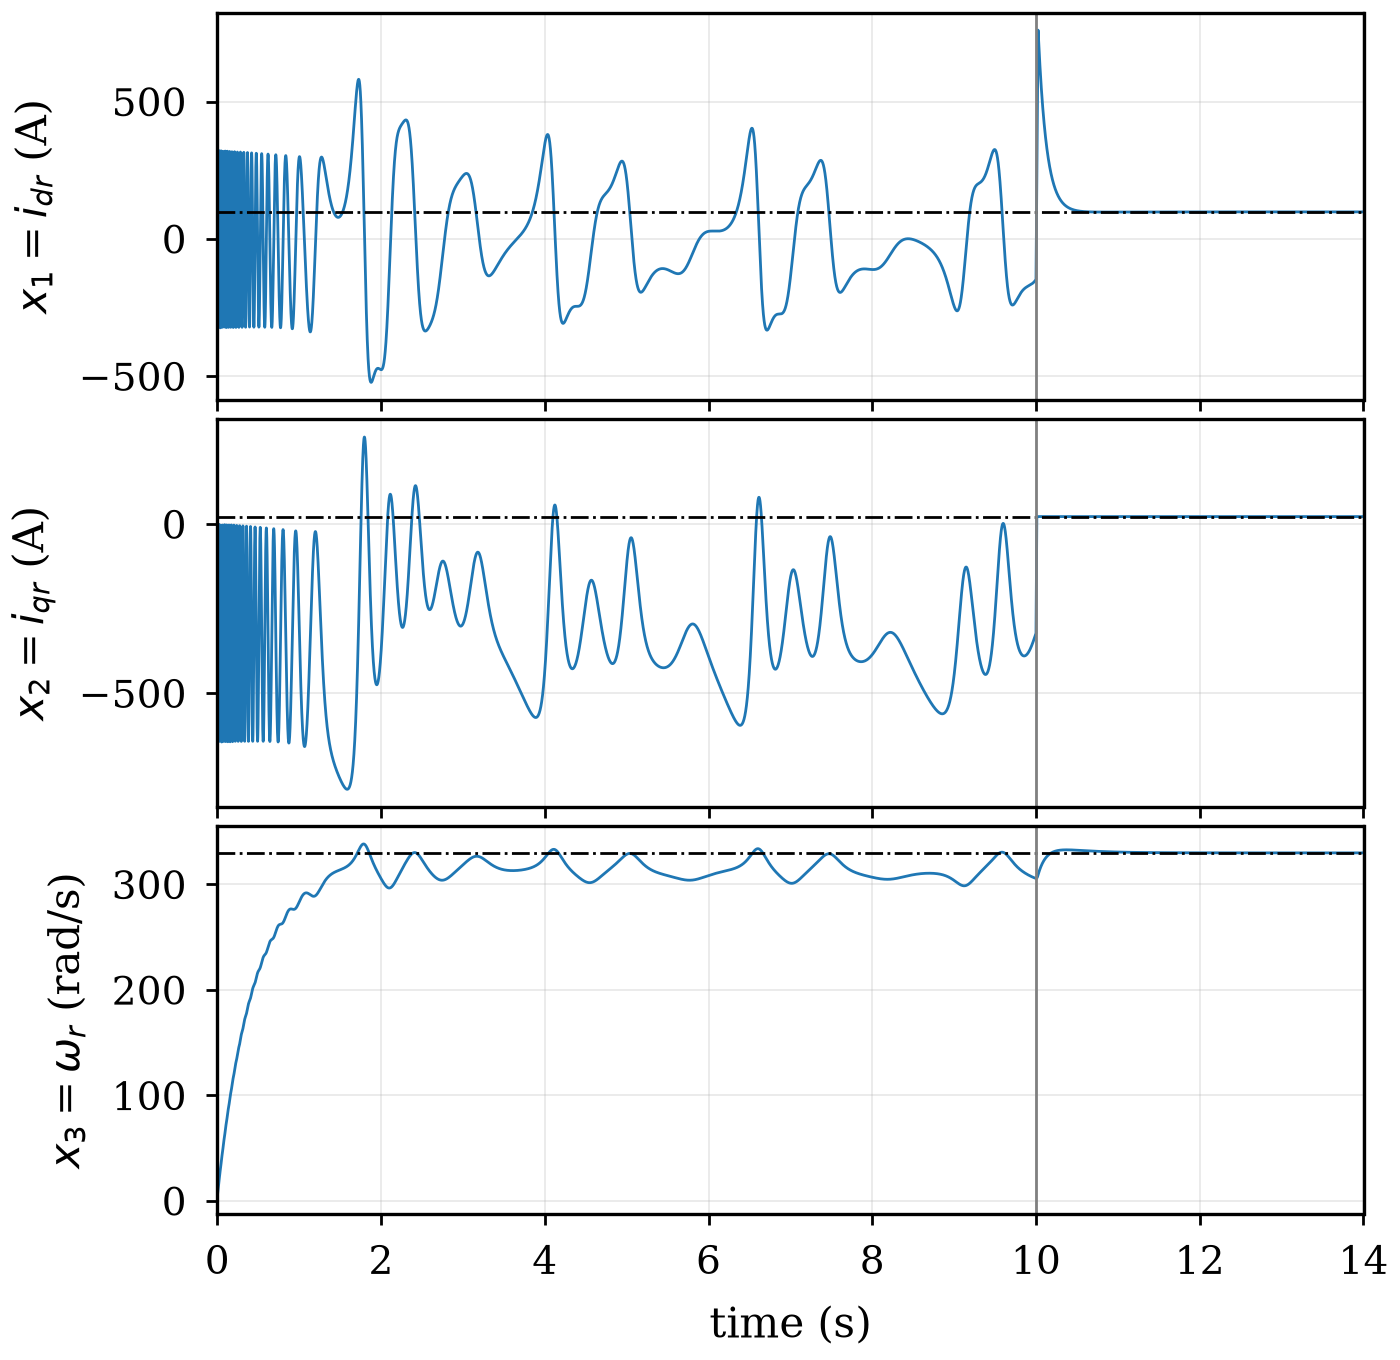
\includegraphics[width=0.48\textwidth]{fig4.png}}
\caption{Time evolution of the state variables before and after control activation at $t=10$~s (dash-dot: target).}
\label{fig4}
\end{figure}

\begin{table}[htbp]
\caption{Chaos Suppression Performance (FL--MPC)}
\begin{center}
\begin{tabular}{|c|c|}
\hline
\textbf{Metric} & \textbf{Value} \\
\hline
IAE of the speed error & 3.63 rad \\
\hline
Settling time (1\,\% band) & 0.13 s \\
\hline
Final speed error & $1.8\times10^{-6}$ rad/s \\
\hline
Steady rotor voltages $u_{dr}$, $u_{qr}$ & 29.3 V, $-8.4$ V \\
\hline
\end{tabular}
\label{tab2}
\end{center}
\end{table}

Fig.~\ref{fig4} shows that the chaotic oscillations disappear as soon as the controller is activated: the speed reaches the positive super-synchronous target and the rotor currents settle at their equilibrium values, using only the rotor voltages. Table~\ref{tab2} shows that the speed enters a 1\,\% band of the target in 0.13~s without steady-state error. During the first instants the rotor voltages reach the 200~V limit, which the MPC accounts for explicitly; afterwards they stay below 34~V and settle at $u_{dr}=29.3$~V, $u_{qr}=-8.4$~V.

\subsection{MPPT Tracking}
For normal operation, the turbine torque $T_{L}=-T_{a}(v,\omega_{r})$ of \eqref{eq3} replaces the constant load, with $R=20$~m, $\lambda_{opt}=8.1$, $C_{p,\max}=0.48$ and $G=86$ in \eqref{eq17} (pole pairs included), and the damping is set to its nominal value $D=0.1$~N$\cdot$m$\cdot$s/rad. The machine is driven by the wind of Fig.~\ref{fig2} (mean 9~m/s); $\omega_{r,ref}$ follows the low-pass filtered wind (time constant 2~s), so that $\omega_{r,ref}$ stays between 279 and 378~rad/s and $P_{s,ref}$ between 142 and 478~kW.

\begin{figure}[htbp]
\centerline{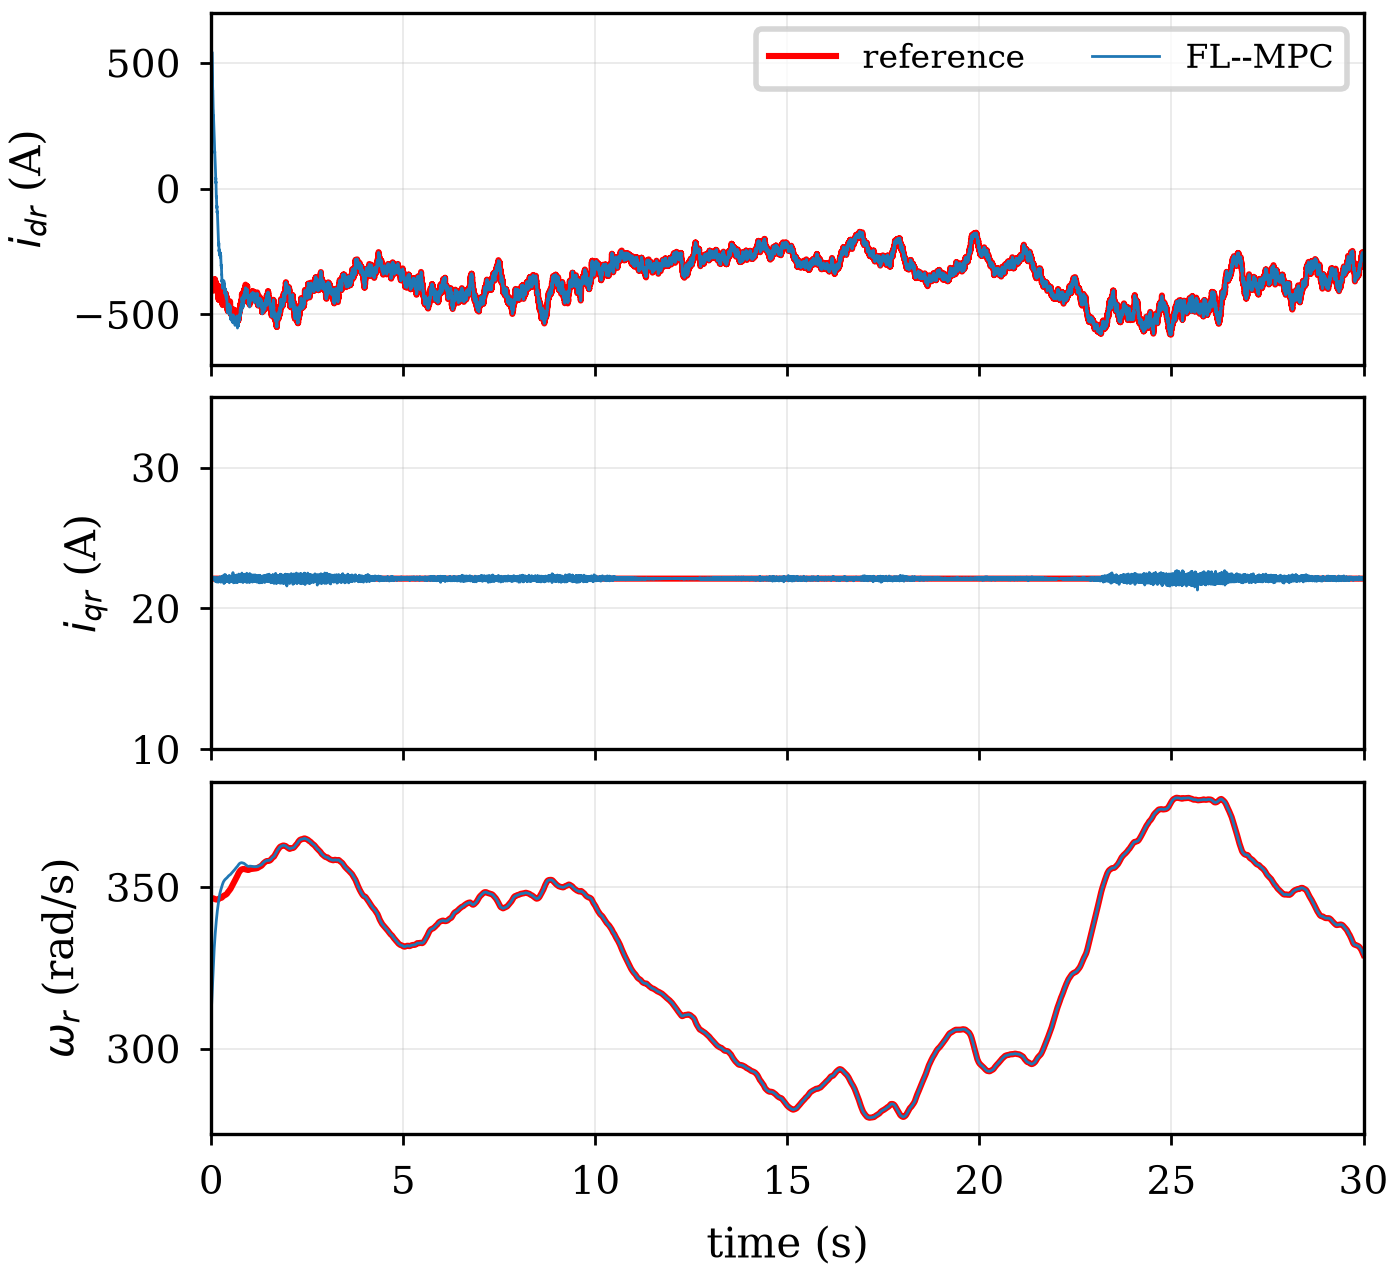
\includegraphics[width=0.48\textwidth]{fig5.png}}
\caption{Tracking performance of the state variables $i_{dr}$, $i_{qr}$, and $\omega_{r}$ under the proposed hybrid control scheme.}
\label{fig5}
\end{figure}

\begin{figure}[htbp]
\centerline{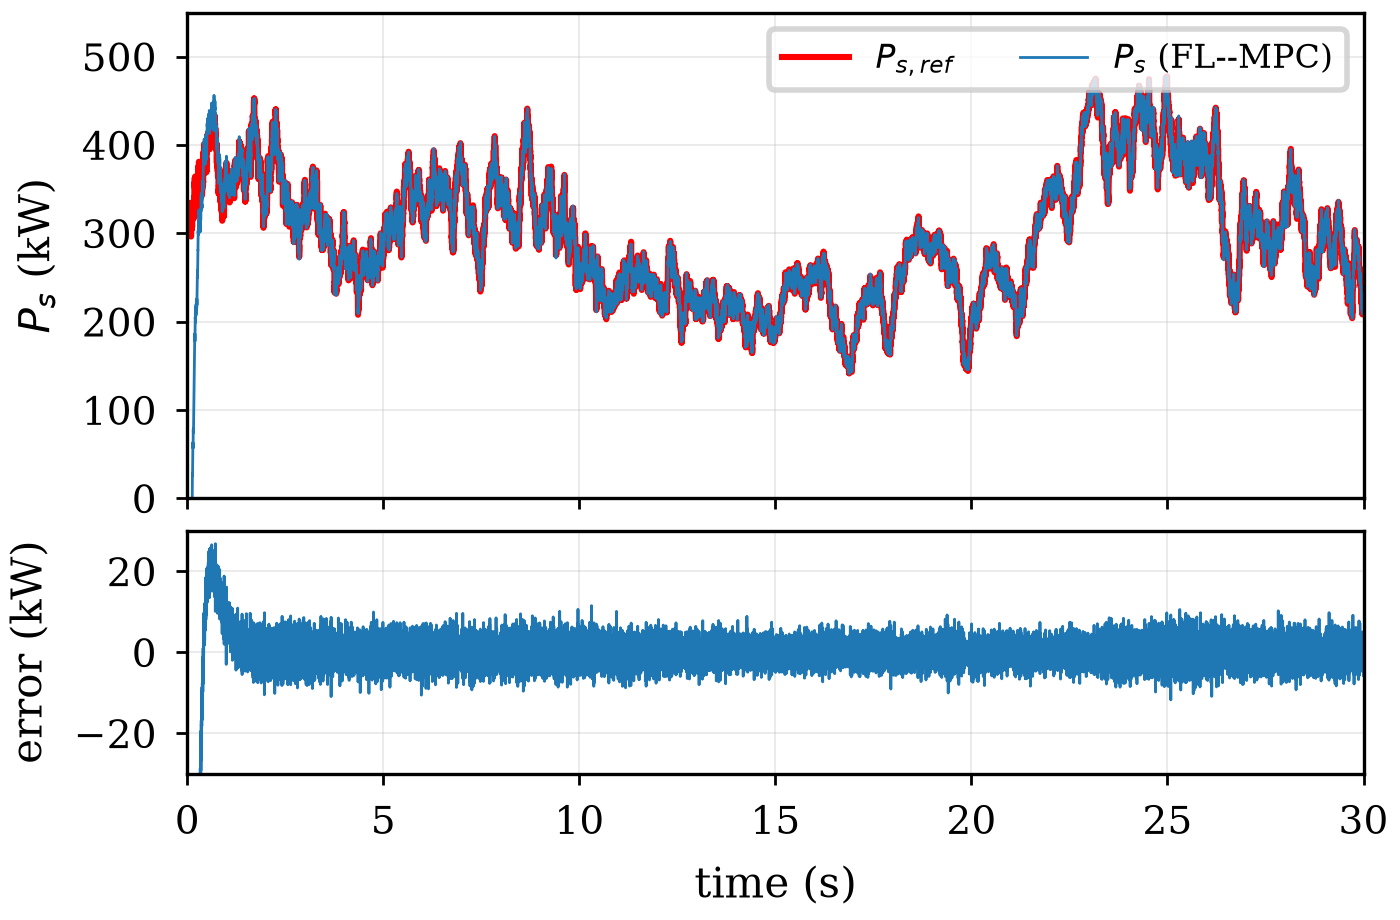
\includegraphics[width=0.48\textwidth]{fig6.png}}
\caption{Active power tracking performance: stator power $P_{s}$ and MPPT reference $P_{s,ref}$, and power tracking error.}
\label{fig6}
\end{figure}

\begin{table}[htbp]
\caption{MPPT Tracking Performance of FL--MPC ($t\ge5$~s)}
\begin{center}
\begin{tabular}{|c|c|}
\hline
\textbf{Metric} & \textbf{Value} \\
\hline
RMS error of $\omega_{r}$ & 0.008 rad/s \\
\hline
RMS error of $i_{dr}$ & 3.28 A \\
\hline
RMS error of $i_{qr}$ & 0.085 A \\
\hline
RMS error of $P_{s}$ & 2.70 kW (0.93\,\% of mean $P_{s}$) \\
\hline
Speed settling time (2\,\% band) & 0.13 s \\
\hline
\end{tabular}
\label{tab3}
\end{center}
\end{table}

Figs.~\ref{fig5} and \ref{fig6} show that $i_{dr}$, $i_{qr}$, $\omega_{r}$ and the stator power follow their MPPT references despite turbulence. Starting from $0.9\,\omega_{r,ref}$, the speed enters a 2\,\% band in 0.13~s. Table~\ref{tab3} shows that the RMS speed error is 0.008~rad/s and the RMS power error 2.70~kW, i.e., below 1\,\% of the mean stator power (291~kW). The voltage limits are reached during start-up and only very briefly afterwards (0.03\,\% of the time, at turbulence peaks); the MPC handles them explicitly, with the stability guarantee of Theorem~1.

\section{Conclusion}

This paper investigated the nonlinear dynamics of a DFIG-based wind energy conversion system with a physically consistent parameter set. The analysis of the equilibria, of the dissipativity and of the Lyapunov exponents confirmed the presence of a chaotic attractor under perturbed parameters. A hybrid controller acting only on the rotor voltages was proposed: an outer speed loop generates the torque-current reference, nonlinear feedback compensation cancels the coupled current dynamics, and a constrained MPC, whose terminal weight and gain are obtained from an LMI, handles the converter voltage limits with guaranteed nominal stability. Simulations show chaos suppression without steady-state error, and accurate MPPT tracking under turbulent wind, with a stator-power RMS error below 1\,\% of the mean power. Future work will address converter and grid dynamics, low-voltage ride-through, and experimental validation.

\section*{Conflict of Interest}
The authors declare there are no conflicts of interest.

\begin{thebibliography}{00}
\bibitem{b1} International Energy Agency (IEA), \textit{World Energy Outlook 2024: Global Energy Demand and Renewable Energy Transition}, Paris, France, 2024. [Online]. Available: https://www.iea.org/reports/world-energy-outlook-2024
\bibitem{b2} International Renewable Energy Agency (IRENA), \textit{Renewable Energy Statistics 2024}, Abu Dhabi, UAE, 2024. [Online]. Available: https://www.irena.org/publications/2024/Jul/Renewable-energy-statistics-2024
\bibitem{b3} United Nations Environment Programme (UNEP), \textit{Emissions Gap Report 2024: The Need for Sustainable Energy Sources}, Nairobi, Kenya, 2024.
\bibitem{b4} Global Wind Energy Council (GWEC), \textit{Global Wind Report 2024: Annual Market Update}, Brussels, Belgium, 2024. [Online]. Available: https://gwec.net/global-wind-report-2024/
\bibitem{b5} International Energy Agency (IEA), \textit{Renewables 2024: Analysis and Forecast to 2028}, Paris, France, 2024. [Online]. Available: https://www.iea.org/reports/renewables-2024
\bibitem{b6} S. Heier, \textit{Grid Integration of Wind Energy: Onshore and Offshore Conversion Systems}, 4th ed. Chichester, UK: Wiley, 2020.
\bibitem{b7} R. Pena, J. C. Clare, and G. M. Asher, ``Doubly fed induction generator using back-to-back PWM converters and its application to variable-speed wind-energy generation,'' \textit{IEE Proc. Electric Power Applications}, vol. 143, no. 3, pp. 231--241, May 1996.
\bibitem{b8} M. G. Simoes and F. A. Farret, \textit{Renewable Energy Systems: Design and Analysis with Induction Generators}, 2nd ed. Boca Raton, FL, USA: CRC Press, 2017.
\bibitem{b9} S. Muller, M. Deicke, and R. W. De Doncker, ``Doubly fed induction generator systems for wind turbines,'' \textit{IEEE Industry Applications Magazine}, vol. 8, no. 3, pp. 26--33, May/Jun. 2002.
\bibitem{b10} A. A. Chhipa, P. Chakrabarti, V. Bolshev, T. Chakrabarti, and G. N. Samarin, ``Modeling and control strategy of wind energy conversion system with grid-connected doubly-fed induction generator,'' \textit{Energies}, vol. 15, no. 18, p. 6694, Sep. 2022.
\bibitem{b11} L. Xu and Y. Wang, ``Dynamic modeling and control of DFIG-based wind turbines under unbalanced network conditions,'' \textit{IEEE Trans. Power Systems}, vol. 22, no. 1, pp. 314--323, Feb. 2007.
\bibitem{b12} A. Tapia, G. Tapia, J. X. Ostolaza, and J. R. Saenz, ``Modeling and control of a wind turbine driven doubly fed induction generator,'' \textit{IEEE Trans. Energy Conversion}, vol. 18, no. 2, pp. 194--204, Jun. 2003.
\bibitem{b13} Y. Lei, A. Mullane, G. Lightbody, and R. Yacamini, ``Modeling of the wind turbine with a doubly fed induction generator for grid integration studies,'' \textit{IEEE Trans. Energy Conversion}, vol. 21, no. 1, pp. 257--264, Mar. 2006.
\bibitem{b14} M. Rahimi and M. Parniani, ``Dynamic behavior and transient stability analysis of fixed speed wind turbines,'' \textit{Renewable Energy}, vol. 34, no. 12, pp. 2613--2624, Dec. 2009.
\bibitem{b15} W. Qiao, G. K. Venayagamoorthy, and R. G. Harley, ``Real-time implementation of a STATCOM on a wind farm equipped with doubly fed induction generators,'' \textit{IEEE Trans. Industry Applications}, vol. 45, no. 1, pp. 98--107, Jan./Feb. 2009.
\bibitem{b16} H. Nian, Y. Song, P. Zhou, and Y. He, ``Improved direct power control of a wind turbine driven doubly fed induction generator during transient grid voltage unbalance,'' \textit{IEEE Trans. Energy Conversion}, vol. 26, no. 3, pp. 976--986, Sep. 2011.
\bibitem{b17} D. Xiang, L. Ran, P. J. Tavner, and S. Yang, ``Control of a doubly fed induction generator in a wind turbine during grid fault ride-through,'' \textit{IEEE Trans. Energy Conversion}, vol. 21, no. 3, pp. 652--662, Sep. 2006.
\bibitem{b18} M. Rahimi and M. Parniani, ``Efficient control scheme of wind turbines with doubly fed induction generators for low-voltage ride-through capability enhancement,'' \textit{IET Renewable Power Generation}, vol. 4, no. 3, pp. 242--252, May 2010.
\bibitem{b19} J. Morren and S. W. H. de Haan, ``Ride-through of wind turbines with doubly-fed induction generator during a voltage dip,'' \textit{IEEE Trans. Energy Conversion}, vol. 20, no. 2, pp. 435--441, Jun. 2005.
\bibitem{b20} M. Tsili and S. Papathanassiou, ``A review of grid code technical requirements for wind farms,'' \textit{IET Renewable Power Generation}, vol. 3, no. 3, pp. 308--332, Sep. 2009.
\bibitem{b21} A. Mechter, K. Kemih, and M. Ghanes, ``Backstepping control of a wind turbine for low wind speeds,'' \textit{Nonlinear Dynamics}, vol. 84, no. 4, pp. 2435--2445, 2016.
\bibitem{b22} A. Mechter, K. Kemih, and M. Ghanes, ``Sliding mode control of a wind turbine with exponential reaching law,'' \textit{Acta Polytechnica Hungarica}, vol. 12, no. 3, pp. 167--183, 2015.
\bibitem{b23} I. Bouguettah, M. Messadi, K. Kemih, \textit{et al.}, ``Adaptive passive fault tolerant control of DFIG-based wind turbine using a self-tuning fractional integral sliding mode control,'' \textit{Frontiers in Energy Research}, vol. 12, p. 1429877, 2024.
\bibitem{b24} S. Regani, M. Messadi, and K. Kemih, ``Modeling and Nonlinear Dynamic Analysis of a DFIG-Based Wind Turbine System,'' submitted to \textit{Journal of Applied Nonlinear Dynamics}, Mar. 2026.
\bibitem{b25} A. Senouci and A. Boukabou, ``Predictive control and synchronization of chaotic and hyperchaotic systems based on a T--S fuzzy model,'' \textit{Mathematics and Computers in Simulation}, vol. 105, pp. 62--78, 2014.
\bibitem{b26} A. Boukabou, A. Chebbah, and N. Mansouri, ``Predictive control of continuous chaotic systems,'' \textit{Int. J. Bifurcation Chaos}, vol. 18, no. 2, pp. 587--592, 2008, doi: 10.1142/S0218127408020501.
\bibitem{b27} M. Messadi and A. Mellit, ``Predictive control of a chaotic permanent magnet synchronous generator in a wind turbine system,'' \textit{Chinese Physics B}, vol. 24, no. 1, p. 010502, 2015.
\bibitem{b28} H. Takhi, L. Moysis, N. Machkour, C. Volos, K. Kemih, and M. Ghanes, ``Predictive control and synchronization of uncertain perturbed chaotic permanent-magnet synchronous generator and its microcontroller implementation,'' \textit{Eur. Phys. J. Spec. Top.}, vol. 231, no. 3, pp. 443--451, 2022, doi: 10.1140/epjs/s11734-021-00422-4.
\bibitem{b29} M. Messadi and A. Mellit, ``Control of chaos in an induction motor system with LMI predictive control and experimental circuit validation,'' \textit{Chaos, Solitons \& Fractals}, vol. 97, pp. 51--58, 2017.
\bibitem{b30} M. Messadi, K. Kemih, and H. Hamiche, ``A new secure communications scheme based on synchronization of hybrid chaotic system,'' \textit{Chaos Theory Appl.}, vol. 5, no. 3, pp. 160--166, 2023, doi: 10.51537/chaos.1276714.
\bibitem{b31} H. Takhi, K. Kemih, L. Moysis, \textit{et al.}, ``Passivity based control and synchronization of perturbed uncertain chaotic systems and their microcontroller implementation,'' \textit{Int. J. Dyn. Control}, vol. 8, no. 3, pp. 973--990, 2020, doi: 10.1007/s40435-020-00618-x.
\bibitem{b32} H. Ren and D. Liu, ``Nonlinear feedback control of chaos in permanent magnet synchronous motor,'' \textit{IEEE Trans. Circuits Syst. II, Exp. Briefs}, vol. 53, no. 1, pp. 45--50, Jan. 2006.
\bibitem{b33} G. Chen, ``A simple adaptive feedback control method for chaos and hyper-chaos control,'' \textit{Applied Mathematics and Computation}, vol. 217, no. 17, pp. 7258--7264, 2011.
\bibitem{b34} P. Jiang, T. Zhang, J. Geng, P. Wang, and L. Fu, ``An MPPT strategy for wind turbines combining feedback linearization and model predictive control,'' \textit{Energies}, vol. 16, no. 10, Art. no. 4244, 2023, doi: 10.3390/en16104244.
\bibitem{b35} D. Q. Mayne, J. B. Rawlings, C. V. Rao, and P. O. M. Scokaert, ``Constrained model predictive control: Stability and optimality,'' \textit{Automatica}, vol. 36, no. 6, pp. 789--814, 2000, doi: 10.1016/S0005-1098(99)00214-9.
\bibitem{b36} M. V. Kothare, V. Balakrishnan, and M. Morari, ``Robust constrained model predictive control using linear matrix inequalities,'' \textit{Automatica}, vol. 32, no. 10, pp. 1361--1379, 1996.
\end{thebibliography}

\end{document}
